\section{Introduction}

Prior to this work, a comprehensive LFG grammar for Turkish had been developed in XLE by \citet{cetinoglu2009}. However, the unavailability of the source files for that implementation necessitated the creation of a small-scale Turkish grammar from scratch for the current implementation.

\begin{sloppypar}
Building grammars in XLE involves two essential steps: formulating c-structure rules and constructing a lexicon with lexical entries. In the present implementation, the Turkish grammar naturally consisted of a small set of c-structure rules and a limited lexicon. Despite its basic nature, the implemented grammar is still of significant size, making it impractical to explore in its entirety within a single chapter. Hence, this chapter will primarily focus on the relevant implementation features related to the analysis presented in the previous chapter. For a comprehensive view of the implementation, readers can refer to Appendix \ref{appendixc:grammar}.
\end{sloppypar}

Furthermore, the verification of the grammar involved extensive testing on sentences representing diverse configurations. The testing process included both well-formed and ill-formed sentences to assess the selectivity of the implementation. A total of 53 sentences were tested, including 22 ill-formed ones. Although providing a detailed analysis of each test sentence is beyond the scope of this chapter, interested readers can find them in Appendix \ref{appendixc:testsentences}.


\section{C-structure rules} \label{sec:cstructure-rules}

The implementation faced a significant challenge in encoding c-structure rules, particularly because the analysis adopted in the previous chapter required the exclusion of syntactic categories represented at node labels, which is a standard XLE implementation feature. To illustrate this, let us consider the rule in (\ref{imp:sentencerule}), which is intended to parse simple Turkish sentences.


\pex
\label{imp:sentencerule}
\vspace{-12pt}

\begin{tabular}{lccc}
	S & $\longrightarrow$ & (NP) & VP \\
	& & ($\uparrow$ \textsc{subj}) = $\downarrow$ & $\uparrow$ = $\downarrow$ \\
	&			   & ($\downarrow$ \textsc{case}) $=_c$ \textsc{nom} &  
\end{tabular}
\xe

This rule posits that a sentence consists of an NP and VP. The NP is identified as the subject of the sentence, and a constraining equation ensures that this position can only be filled by a nominative NP. Crucially, the NP can be omitted (as indicated by parentheses) since the inclusion of the subject is optional in Turkish. 

However, according to the analysis proposed by \citet{prz:pat:21:oup}, this rule has to be modified, as shown in (\ref{imp:sentencerule1}).

\pex
\vspace{-12pt}
\label{imp:sentencerule1}

\begin{tabular}{lccc}
	S & $\longrightarrow$ & (XP) & XP \\
	& & ($\uparrow$ \textsc{subj}) = $\downarrow$ & $\uparrow$ = $\downarrow$ \\
	&			   & ($\downarrow$ \textsc{case}) $=_c$ \textsc{nom} & ($\downarrow$ \textsc{cat}) =$_c$ V  \\
	& & ($\downarrow$ \textsc{cat}) =$_c$ N &  \\
\end{tabular}
\xe

The XLE version of the sentence rule, as presented in (\ref{imp:sentencexle}), is not vastly different from the original LFG rule. However, some elucidation is still needed to explain the parallelisms between LFG and XLE notations.

\pex
\label{imp:sentencexle}
\vspace{-18pt}

\lstset{
	escapeinside={(*@}{@*)}, basicstyle=\small\ttfamily
}
\begin{lstlisting}
	S -->   (X_MAX: (^ SUBJ) = !
	  		(! CASE) =c NOM)
			(! CAT) =c N
			
		 X_MAX: ^=!
			(! CAT) =c V.
\end{lstlisting}
\xe

In XLE notation, functional annotations are not located below their respective nodes, as is typical in standard LFG rules. Instead, functional annotations are attached to their nodes using the semicolon placed next to the node labels. The metavariables $\uparrow$ and $\downarrow$ in LFG notation are represented in XLE by the caret symbol (\texttt{\^}) and exclamation mark (\texttt{!}), respectively. It is worth mentioning that in XLE, there is no need to explicitly signify conjunction ($\land$) through symbols such as \texttt{\&}. Instead, the conjunction between constraints (or functional equations) is implied when they are placed adjacent to each other. In this instance, despite there being no conjunction symbols between functional equations, XLE interprets them as logical conjuncts. Additionally, the presented XLE rule encodes XP as \texttt{X\_MAX} since the implemented grammar followed a notation that used \texttt{X\_n} to represent bar-levels, with \texttt{X\_1} representing X$'$ and \texttt{X\_0} representing X.

When it comes to coordination rule, the most straightforward way of encoding it would be as follows: 

\pex
\vspace{-12pt}
\label{imp:coordrule0}

\begin{tabular}{lcccc}
	XP & $\longrightarrow$ & XP$^{+}$ & X & XP \\
	& & $\uparrow$ $\in$ $\downarrow$ & $\uparrow$ = $\downarrow$ & $\uparrow$ $\in$ $\downarrow$ \\
	& & & ($\downarrow$ \textsc{cat}) =$_c$ CNJ & 
\end{tabular}
\xe

In this representation, the rule does not impose constraints on the syntactic categories of the conjuncts, as such constraints depend on the specific syntactic position they occupy. However, the head of the phrase (coordination) is constrained to have the category CNJ. When transferred to XLE, this rule would be expressed as in (\ref{imp:xlecoord0}).

\newpage
\pex
\label{imp:xlecoord0}
\vspace{-19pt}

\lstset{
	escapeinside={(*@}{@*)}, basicstyle=\small\ttfamily
}
\begin{lstlisting}
	X_MAX --> X_MAX+: ! $ ^;
	          X: ^ = !
	             (! CAT) =c CNJ
	          X_MAX: ! $ ^.
\end{lstlisting}
\xe

However, this rule clashed with other \texttt{X\_MAX} rules (see Appendix \ref{appendixc:c-structure} for other \texttt{X\_MAX} rules) for different phrase types, for reasons that remain unclear. Consequently, the grammar failed to produce parses for sentences containing coordination. To overcome this issue, the rule had to be adapted as shown in (\ref{imp:xlecoord1}). Importantly, this modification does not imply that the current thesis asserts coordination to have the category COORD. Rather, the rule should be interpreted solely as a technical workaround.

\pex
\label{imp:xlecoord1}
\vspace{-19pt}

\lstset{
	escapeinside={(*@}{@*)}, basicstyle=\small\ttfamily
}
\begin{lstlisting}
	COORD --> X_MAX+: ! $ ^;
		  CNJ: ^ = !;
		  X_MAX: ! $ ^.
\end{lstlisting}
\xe

\section{Coordination of unlike adjuncts}
\subsection{Verbal adjuncts}

In the previous section, it was put forward that coordination of unlike verbal adjuncts can be best accounted for through c-structure rules rather than at the level of lexical entries. The XLE representation of the rule (\ref{imp: adjverbal_rule2}) is provided in (\ref{imp:adjrulexle}).

\pex
\vspace{-12pt}

\label{imp: adjverbal_rule2}
\begin{tabular}{lccc}
	X$'$ & $\longrightarrow$ & XP$^{+}$ & X$'$ \\
	& & $\downarrow$ $\in$ ($\uparrow$ \textsc{adj}) & $\uparrow$ = $\downarrow$ \\
	&			   & ($\downarrow$ \textsc{cat}) $\in_{c}$ \{P, N, Adv\} & ($\downarrow$ \textsc{cat}) =$_{c}$ V  
\end{tabular}
\xe

\pex
\vspace{-18pt}
\label{imp:adjrulexle}

\lstset{
	escapeinside={(*@}{@*)}, basicstyle=\small\ttfamily
}
\begin{lstlisting}
	X_MAX --> {	"VP"
			{
			"Verbal adjuncts"
			(COORD: ! $ (^ ADJUNCT)
				(! CAT) $ {P N ADV})
			|
			(X_MAX: ! $ (^ ADJUNCT)
				(! CAT) $ {P N ADV})
			}
			"Verbal head"
			X_1: ^=!
			     (! CAT) =c V
\end{lstlisting}
\xe

It is worth noting that there are some differences between the original formulation and the XLE representation. First, \texttt{X\_MAX} is used as the mother node instead of X$'$ (\texttt{X\_1}) and the verbal adjuncts are marked as optional elements instead of being adorned with Kleene plus. This decision was made to keep c-structure rules and testing as simple as possible.  Second, the verbal adjunct position preceding the verbal head is allowed to rewrite either to \texttt{COORD} or a single \texttt{X\_MAX} (indicated by the use of " | "). This is due to coordination being encoded as a separate rule rather than being part of the \texttt{X\_MAX} rules.

Now, let us put our grammar to the test and examine how it handles different instances of verbal adjuncts. Consider the sentences provided in (\ref{adj-verbaltest}), which allow us to test different configurations for the implemented analysis.

\pex[glspace=!1em,everygla={},everyglb={},aboveglbskip=-.15ex, interpartskip=15pt]
\label{adj-verbaltest}
\a\label{adj-verbaltesta} 
\begingl
\gla\ljudge{*}Kural-lar-a göre ve zor çalış-ıyor-uz. //
\glb rule-\textsc{pl}-\textsc{dat} {according to} and difficult work-\textsc{pres.prog}-\textsc{1pl} //
\glft `We work according to the rules and hard.' //
\endgl
\a\label{adj-verbaltestb} 
\begingl
\gla Yürü-yerek veya tekne-ler ile merkez-e ulaş-ır-sın. //
\glb walk-\textsc{advz} or boat-\textsc{pl} with center-\textsc{dat} reach-\textsc{aor}-\textsc{2sg} //
\glft `(You) reach the center on foot or by boats.' //
\endgl
\a\label{adj-verbaltestc} 
\begingl
\gla Yürü-yerek ve yorul-madan merkez-e ulaş-ır-sın. //
\glb walk-\textsc{advz} and {be tired}-\textsc{advz} center-\textsc{dat} reach-\textsc{aor}-\textsc{2sg} //
\glft `(You) reach the center on foot and without getting tired.' //
\endgl
\xe 

The sentence (\ref{adj-verbaltesta}) is ungrammatical as coordinating a PP with an AdjP violates the rule in (\ref{imp:adjrulexle}). Thus, XLE should not produce a parse for this sentence. Similarly, (\ref{adj-verbaltestb}) features a coordination of unlike verbal adjuncts, where the first conjunct, \textit{belediyeyle birlikte}, is a PP, and the second conjunct, \textit{yorulmadan}, is an AdvP. The implemented grammar, however, should correctly parse this sentence, as PPs and AdvPs can be coordinated in the verbal adjunct position. Finally, the sentence (\ref{adj-verbaltestc}) contains a coordination of two adverbs that modify the predicate \textit{ulaşırsın} `you reach'. This sentence should be recognized as a licit structure by our grammar, as it represents a standard coordination of adverbs.


As expected, XLE fails to produce a parsing solution for the first sentence, as the category of the second conjunct does not satisfy the functional annotation \mbox{\texttt{(!\ CAT) \$ \{P N ADV\})}}. However, for the second sentence (\ref{adj-verbaltestb}), XLE successfully generates both the correct c-structure (Figure \ref{fig:cstr-vadj}) and f-structure (Figure \ref{fig:fstrverbadj}). The coordinated elements are identified as verbal adjuncts and they differ in their \textsc{cat} value. For the third sentence, a similar parse is obtained, with the exception that both adjunct conjuncts have the same \textsc{cat} value.


\vspace{10pt}


\begin{figure}[H]
	\centering
	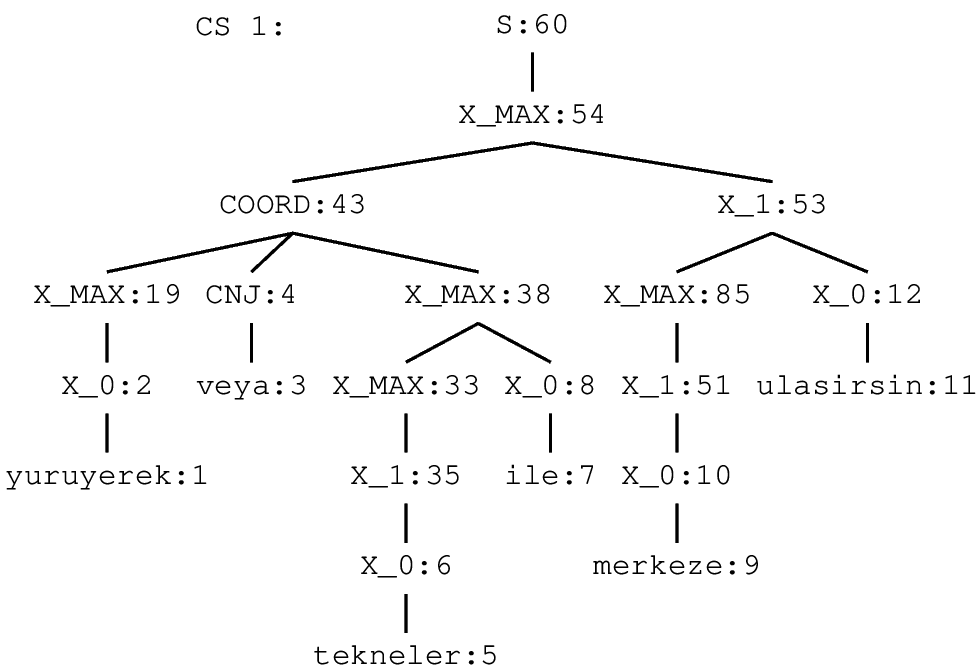
\includegraphics[width=0.72\linewidth]{images/implementation/cstr:verbadj}
	\caption{XLE screenshot of c-structure of sentence (\ref{adj-verbaltestb})}
	\label{fig:cstr-vadj}
\end{figure}

\begin{figure}[H]
	\centering
	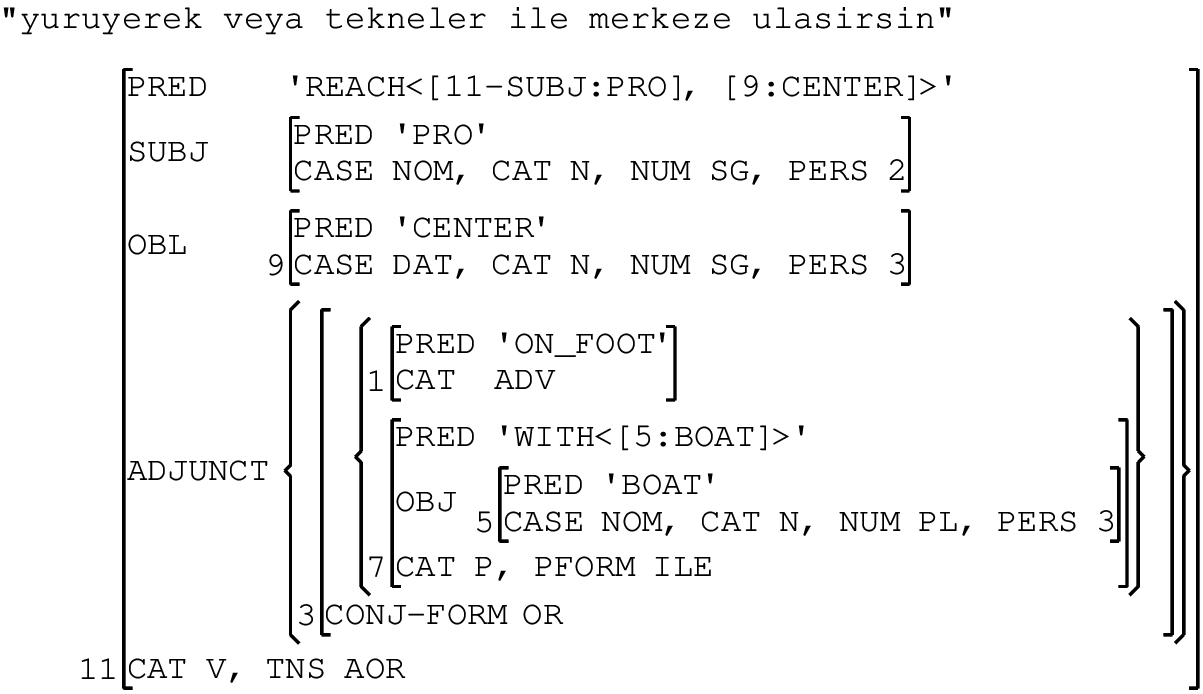
\includegraphics[width=0.7\linewidth]{images/implementation/fstr:verbadj}
	\caption{XLE screenshot of f-structure of sentence (\ref{adj-verbaltestb})}
	\label{fig:fstrverbadj}
\end{figure}

\subsection{Nominal adjuncts}

\begin{sloppypar}
The implementation of the rule governing nominal adjuncts is structurally quite similar to the one for verbal adjuncts, as both types of adjuncts are constrained through their c-structure positions. The rule proposed in the analysis chapter (repeated here in (\ref{imp:adjnom_rule2})) is transferred to XLE as shown in (\ref{imp:adjnomrulexle}). In this rule, the head of the phrase is constrained to be a nominal, as indicated by \mbox{\texttt{(!\ CAT) =c N}}, and the adjuncts can only be either a PP or an AdjP, as indicated by \mbox{\texttt{(!\ CAT) \$ \{P A\}}}.
\end{sloppypar}

\pex
\vspace{-13pt}

\label{imp:adjnom_rule2}
\begin{tabular}{lccc}
	X$'$ & $\longrightarrow$ & XP$^{+}$ & X$'$ \\
	& & $\downarrow$ $\in$ ($\uparrow$ \textsc{adj}) & $\uparrow$ = $\downarrow$ \\
	&			   & ($\downarrow$ \textsc{cat}) $\in_{c}$ \{P, Adj\} & ($\downarrow$ \textsc{cat}) =$_{c}$ N  
\end{tabular}
\xe

\newpage 
\pex
\vspace{-19pt}
\label{imp:adjnomrulexle}

\lstset{
	escapeinside={(*@}{@*)}, basicstyle=\small\ttfamily
}
\begin{lstlisting}
	X_MAX --> {	"NP"
		        {
			"Nominal adjuncts"
			(COORD:! $ (^ ADJUNCT)
				 (! CAT) $ {P A})
			|
			(X_MAX: ! $ (^ ADJUNCT)
				 (! CAT) $ {P A})		
		        }
		        "Nominal head"
		        X_1: ^=!
		             (! CAT) =c N }
	\end{lstlisting}
	\xe

Let us now test this rule on different configurations provided in (\ref{adj-nominaltest}). The first sentence (\ref{adj-nominaltesta}) is ungrammatical because the nominal adjunct position is occupied by a coordination of AdjP and AdvP, which is not permitted according to the rule. However, the sentence (\ref{adj-nominaltestb}) incorporates a coordination of a PP and an AdjP, which should be correctly parsed by the grammar. Finally, the last sentence involves a coordination of AdjPs, which should also not pose a problem for the grammar.

\pex[glspace=!1em,everygla={},everyglb={},aboveglbskip=-.15ex, interpartskip=15pt]
\label{adj-nominaltest}
\a\label{adj-nominaltesta} 
\begingl
\gla\ljudge{*}Güzel ve profesyonel-ce eser-ler-i konuş-tu-k. //
\glb beautiful and professional-\text{advz} work-\textsc{pl}-\textsc{acc} talk-\textsc{pst}-\textsc{1pl} //
\glft `(We) talked about beautiful and professionally works of art.' //
\endgl
\a\label{adj-nominaltestb} 
\begingl
\gla Antik dönem-e ait ve eskimiş eser-ler-i konuş-tu-k. //
\glb antiquated era-\textsc{dat} {belong to} and obsolescent work-\textsc{pl}-\textsc{acc} talk-\textsc{pst}-\textsc{1pl} //
\glft `(We) talked about works of art that belong to ancient history and are obsolescent' //
\endgl
\a\label{adj-nominaltestc} 
\begingl
\gla Güzel ve antik enstrüman-lar-ı konuş-tu-k. //
\glb beautiful and antiquated instrument-\textsc{pl}-\textsc{acc} talk-\textsc{pst}-\textsc{1pl}  //
\glft `(We) talked about beautiful and antiquated instruments.' //
\endgl
\xe 

The first sentence (\ref{adj-nominaltesta}) does not receive a parsing solution, as the nominal adjunct position is occupied by a coordination of an AdjP and an AdvP, which is not permitted. The second sentence (\ref{adj-nominaltestb}) receives the desired parsing solution, as indicated by its c-structure (Figure \ref{fig:cstr-nomadj1}) and f-structure (Figure \ref{fig:fstrnomadj1}).\footnote{The grammar produces another solution for (\ref{adj-nominaltestb}) where \textit{antik} `antiquated' is parsed as one of the conjuncts rather than the adjectival modifier of \textit{döneme} `era'. This alternative reading is indeed easily recoverable in spoken language if a prosodic break (i.e., a pause) is inserted between \textit{antik} and \textit{döneme}.} The last sentence (\ref{adj-nominaltestc}) is also correctly parsed.


\begin{figure}[H]
	\centering
	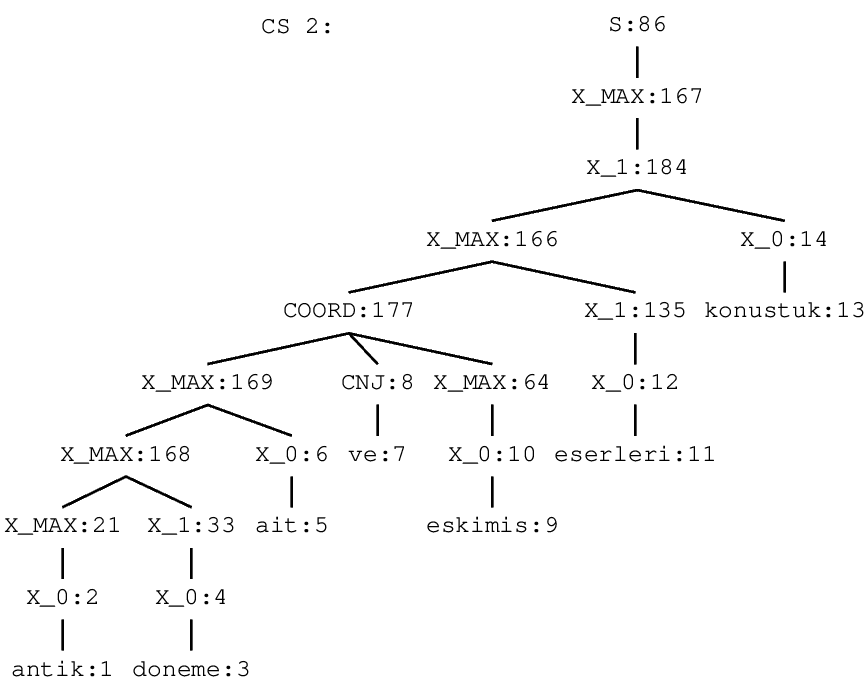
\includegraphics[width=0.7\linewidth]{images/implementation/cstr:nomadj1}
	\caption{XLE screenshot of c-structure of sentence (\ref{adj-nominaltestb})}
	\label{fig:cstr-nomadj1}
\end{figure}

\begin{figure}[H]
	\centering
	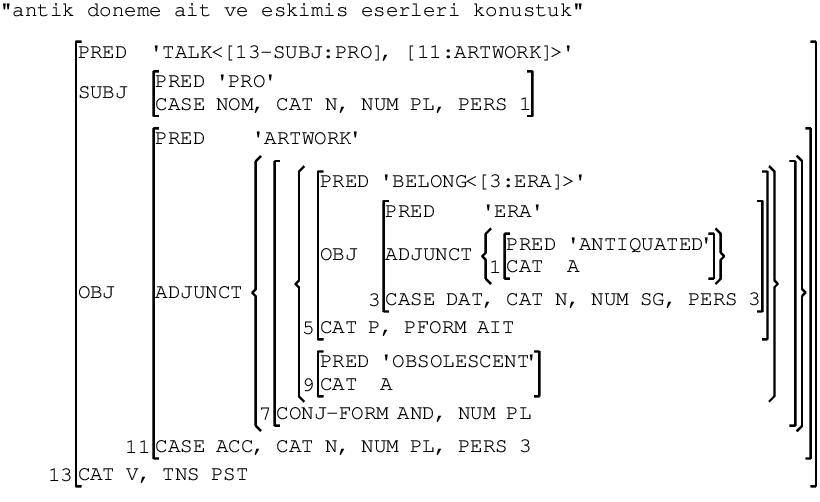
\includegraphics[width=0.73\linewidth]{images/implementation/fstr:nomadj1}
	\caption{XLE screenshot of f-structure of sentence (\ref{adj-nominaltestb})}
	\label{fig:fstrnomadj1}
\end{figure}

\section{Implementing the conservative solution}
\subsection{Off-path constraints}

In the preceding chapter, among the analyses offered by \citeauthor{prz:pat:21:oup}, the choice was made to embrace the liberal solution when formally analyzing Turkish unlike coordination, due to its conceptual advantages. In contrast to the liberal solution, the conservative solution offers the capacity to enforce morphosyntactic constraints on the f-structure of individual conjuncts without extending the formalism of LFG. While the conservative solution involves more complicated formal machinery, it is fully compatible with XLE, making it the ideal option for implementation.

The conservative solution relies on using a specific constraint type called off-path constraints. Before demonstrating their application, consider the examples (\ref{offpath1}) and (\ref{offpath2}) to understand the basic mechanism of off-path constraints on f-structures.

\noindent
\begin{minipage}{0.5\textwidth}
	\pex
	\label{offpath1}
	\a\label{offpath1.constraint}($\uparrow$ \qquad \textsc{a} \qquad \textsc{b} \hspace{5pt} \textsc{c}) =$_{c}$ $+$ \\ \hspace*{0.75em} ($\leftarrow$ \textsc{d}) =$_{c}$ \textsc{e}  
	\a\label{offpath1.fstructure}\begin{avm}
		\[ A \quad \[ 
		B \quad \[ 
		C & + \] 
		\] \\
		D \quad E
		\]
	\end{avm}
	\xe
\end{minipage}
\hfill
\begin{minipage}{0.5\textwidth}
	\pex
	\label{offpath2}
	\a\label{offpath2.constraint}($\uparrow$ \qquad \textsc{a} \qquad \textsc{b} \hspace{5pt} \textsc{c}) =$_{c}$ $+$ \\ \hspace*{0.75em} ($\rightarrow$ \textsc{d}) =$_{c}$ \textsc{e} 
	\a\label{offpath2.fstructure}
	\begin{avm}
		\[ A \quad \[ 
		B \quad \[ 
		C & + \] \\
		D \quad E 
		\]
		
		\]
	\end{avm}
	\xe
\end{minipage}

The constraints themselves can be observed in (\ref{offpath1.constraint}) and (\ref{offpath2.constraint}). The minimal f-structures that satisfy them are given in (\ref{offpath1.fstructure}) and (\ref{offpath2.fstructure}), respectively. The first lines of the constraints are simply constraining equations. The second lines of the constraints, however, are where the off-path constraints are found, which are placed directly below the attribute that they apply. 

Crucially, off-path constraints use distinct metavariables in the form of horizontal arrows. The left arrow ($\leftarrow$) denotes the f-structure that contains the attribute that the off-path constraint applies. The right arrow ($\rightarrow$), on the other hand, refers to the the value of the attribute that the off-path constraint applies. 

In both examples, although the off-path constraint is assigned to the attribute \textsc{a}, they use different horizontal arrows. In (\ref{offpath1.constraint}), the use of $\leftarrow$ states that there must be an attribute-value pair $\langle$\textsc{d, e}$\rangle$ in the f-structure that contains the attribute \textsc{a}, which is satisfied by the f-structure in (\ref{offpath1.fstructure}). In (\ref{offpath2.constraint}), $\rightarrow$ that the attribute-value pair $\langle$\textsc{d, e}$\rangle$ must instead be found in the f-structure that corresponds to the value of the attribute \textsc{a}.

\subsubsection{From distributive statements to off-path constraints}

As previously discussed, he liberal solution proposed by P\&P involves extending the definition of distributivity to constraining statements. The original statement that they proposed for the constraints imposed by \textit{believe} on its oblique argument is shown again in (\ref{przpat:statement1}).

\ex
\label{przpat:statement1}
($\uparrow$ \textsc{obl}) = \%\textsc{c} $\land$ \\
\vspace{3pt}\text{[[}(\%\textsc{c cat}) =$_c$ V $\land$ (\%\textsc{c comp-form}) =$_c$ \textsc{that}] $\lor$ \\
\text{[}(\%\textsc{c cat}) =$_c$ P $\land$ (\%\textsc{c pform}) =$_c$ \textsc{in}\text{]]}
\xe

This statement can be ``translated'' to an off-path constraint to achieve the same effect, as shown below.


\ex
( $\uparrow$  \textsc{obl} \hspace*{9em} \textsc{pred} \hspace*{9.5em}) \\
\hspace*{3em} \{($\leftarrow$ \textsc{cat}) =$_{c}$ V \hspace*{0.5em} $\land$ \hspace*{0.5em} [($\leftarrow$ \textsc{comp-form}) =$_{c}$ \textsc{that} \\
\hspace*{4em} $\lor$ [($\leftarrow$ \textsc{cat}) =$_{c}$ P \hspace*{0.5em} $\land$ \hspace*{0.5em} ($\leftarrow$ \textsc{pform}) =$_{c}$ \textsc{in}]
\xe

Within the context of this off-path constraint, $\leftarrow$ refers to the f-structure of the oblique argument of \textit{believe}. Once this off-path constraint is added to lexical entry for \textit{believe}, the \textsc{obl} argument of \textit{believe} can be either a CP projected by \textit{that}, as indicated by the \textsc{comp-form} attribute, or a PP projected by \textit{in}, as indicated by the \textsc{pform} attribute. The constraint is anchored to the \textsc{pred} attribute, as any lexical item mapped to the \textsc{obl} attribute inherently carries its respective \textsc{pred} attribute. This anchoring ensures that the off-path constraint is evaluated for each f-structure containing \textsc{pred} if the \textsc{obl} attribute is mapped to a hybrid object corresponding to coordination. In other words, this constraint is recycled for each conjunct, as each conjunct has the \textsc{pred} attribute. 


\section{Coordination of unlike arguments}
\subsection{Predicative arguments}

In the previous chapter, the morphosyntactic restrictions imposed by the Turkish verb \textit{ol-} 'be/become' upon its predicative arguments were formulated as a distributive constraint (see (\ref{pred-liberal})). This distributive formulation can be converted into an off-path constraint, as demonstrated in (\ref{pred-offpath}).

\ex
\label{pred-liberal}
($\uparrow$ \textsc{predlink}) = \%\textsc{c} $\land$ \\
\vspace{3pt}\text{[[}(\%\textsc{c cat}) =$_c$ N $\land$ $\neg$\text{[}(\%\textsc{c case}) =$_c$ \textsc{acc} $\lor$ (\%\textsc{c case}) =$_c$ \textsc{dat}\text{]]} $\lor$ \\
(\%\textsc{c cat})  =$_c$ P $\lor$ \\
(\%\textsc{c cat})  =$_c$ Adj\text{]]}
\xe

\ex
\label{pred-offpath}
( $\uparrow$  \textsc{predlink} \hspace*{12em} \textsc{pred} \hspace*{12.8em}) \\
\hspace*{5.3em} \{($\leftarrow$ \textsc{cat}) =$_{c}$ N \hspace*{0.4em} $\land$ \hspace*{0.4em} $\neg$[($\leftarrow$ \textsc{case}) =$_{c}$ \textsc{acc} \hspace*{0.2em} $\lor$ \hspace*{0.2em} ($\leftarrow$ \textsc{case}) =$_{c}$ \textsc{dat}]\}
\\
\hspace*{9.5em} $\lor$ \hspace*{0.4em} [($\leftarrow$ \textsc{cat}) =$_{c}$ P \hspace*{0.4em} $\lor$ \hspace*{0.4em} ($\leftarrow$ \textsc{cat}) =$_{c}$ Adj]
\xe

This off-path constraint states that for each \textsc{pred} containing f-structure that is the value of the \textsc{predlink} attribute, exactly one of the following conditions must be satisfied:

\begin{itemize}
	\item It must contain a \textsc{cat} attribute with the value N (representing nominal category), and it must \textbf{not} possess the attribute-value pairs $\langle$\textsc{case, acc}$\rangle$ or $\langle$\textsc{case, dat}$\rangle$.
	\item It must contain a \textsc{cat} attribute with the value P (representing postpositional category).
	\item It must contain a \textsc{cat} attribute with the value Adj (representing adjectival category).
\end{itemize}

The XLE implementation of the constraint, as shown in (\ref{imp:xleol}), utilizes specific notations to represent various linguistic features. Notably, XLE employs the notation \texttt{<-} to signify the leftward pointing horizontal arrow ($\leftarrow$), establishing the connection between the f-structure(s) and the \textsc{predlink} argument. Additionally, the negation symbol ``$\neg$'' is represented in XLE using the tilde symbol ``$\sim$''. As previously mentioned, XLE interprets the adjacency (as indicated by the space) between statements as an indication of logical conjunction, which renders \mbox{``($\leftarrow$ \textsc{cat}) =${c}$ N''} and \mbox{``$\neg$[($\leftarrow$ \textsc{case}) =${c}$ \textsc{acc} $\lor$ ($\leftarrow$ \textsc{case}) =$_{c}$ \textsc{dat}''} as logical conjuncts. Furthermore, the entire disjunctive constraint is anchored to the \texttt{PRED} attribute through the use of a semicolon adjacent to the \texttt{PRED} attribute.
\newpage
\pex
\vspace{-20pt}
\label{imp:xleol}

\lstset{
	escapeinside={(*@}{@*)}, basicstyle=\small\ttfamily
}

\begin{lstlisting}
    (^ PREDLINK PRED: 
    {(<- CAT) =c N ~{(<- CASE) =c ACC | (<- CASE) =c DAT} | 
    (<- CAT) =c P | 
    (<- CAT) =c A}).
\end{lstlisting}
\xe


This constraint has demonstrated its effectiveness in handling distinct configurations represented by a total of specifically designed 9 test sentences. For well-formed sentences, the grammar correctly provides valid parses, and, in the case of ill-formed strings, the grammar behaves as expected by not providing any solutions.

\subsection{Object arguments}

The verb \textit{konuş-} `talk/converse' imposes intricate morphosyntactic constraints on its object(s). These constraints were captured in the preceding chapter using the subsequent distributive constraining statement:

\ex
\label{obj-liberal}
($\uparrow$ \textsc{obj}) = \%\textsc{c} $\land$ \\
\vspace{3pt}\text{[[}(\%\textsc{c cat}) =$_c$ P $\land$ \text{[}(\%\textsc{c pform}) =$_c$ \textsc{hakkinda} $\lor$ (\%\textsc{c pform}) =$_c$ \textsc{üzerine}\text{]]} $\lor$ \\
\text{[}(\%\textsc{c cat}) =$_c$ N $\land$ \text{[}(\%\textsc{c case}) =$_c$ \textsc{acc} $\lor$ (\%\textsc{c case}) =$_c$ \textsc{nom}\text{]]]}
\xe

This constraining statement can be equivalently transformed into the following off-path constraint:

\ex
\label{obj-conservative}
( $\uparrow$  \textsc{obj} \hspace*{12em} \textsc{pred} \hspace*{16em})
\\
\hspace*{1.5em} [($\leftarrow$ \textsc{cat}) =$_{c}$ P \hspace*{0.2em} $\land$ [($\leftarrow$ \textsc{pform}) =$_{c}$ \textsc{hakkında} $\lor$ \hspace*{0.2em} ($\leftarrow$ \textsc{pform}) =$_{c}$ \textsc{üzerine}]] \\
\hspace*{3.5em} $\lor$  \{($\leftarrow$ \textsc{cat}) =$_{c}$ N \hspace*{0.2em} $\land$ \hspace*{0.2em} [($\leftarrow$ \textsc{case}) =$_{c}$ \textsc{acc} $\lor$ ($\leftarrow$ \textsc{case}) =$_{c}$ \textsc{nom}]\} 
\xe

This off-path constraint stipulates that for each \textsc{pred} containing f-structure that is the value of the \textsc{obj} attribute, exactly one of the following constraints must hold:

\begin{sloppypar}
	\begin{itemize}
		\item It must contain a \textsc{cat} attribute with the value P, and it must either possess the attribute-value pair $\langle$\textsc{pform, hakkında}$\rangle$ or $\langle$\textsc{pform, üzerine}$\rangle$.
		\item It must contain a \textsc{cat} attribute with the value N, and it must possess either the attribute-value pair $\langle$\textsc{case, acc}$\rangle$ or $\langle$\textsc{case, nom}$\rangle$.
	\end{itemize}
\end{sloppypar}

The corresponding XLE implementation of this constraint is presented below:

\pex
\label{imp:xlekonuş_modified}
\vspace{-18pt}

\lstset{
	escapeinside={(*@}{@*)}, basicstyle=\small\ttfamily
}
\begin{lstlisting}
    (^ OBJ PRED:
    {(<- CAT) =c N {(<- CASE) =c ACC | (<- CASE) =c NOM} |
    (<- CAT) =c P {(<- PFORM) =c HAKKINDA 
    | (<- PFORM) =c UZERINE}}).
\end{lstlisting}
\xe

The effectiveness of this constraint was verified through testing on 8 different configurations (sentences), where it demonstrated its capability to handle them effectively.

\subsection{Oblique arguments}

Coordination uf unlike oblique arguments was examined in the previous chapter within the context of two verbs: \textit{saydır-} `curse/swear' and sür- `last/continue'.

The morphosyntactic constraints imposed by the verb \textit{saydır-} on its oblique argument was formulated through the distributive statement in (\ref{obl-liberal}), which is translated into the off-path constraint in (\ref{obl-cons}).

\ex
\label{obl-liberal}
($\uparrow$ \textsc{obl}) = \%\textsc{c} $\land$ \\
\vspace{3pt}\text{[[}(\%\textsc{c cat}) =$_c$ N $\land$ (\%\textsc{c case}) =$_c$ \textsc{dat}\text{]} $\lor$ \\
\text{[}(\%\textsc{c cat}) =$_c$ P $\land$ (\%\textsc{c pform}) =$_c$ \textsc{hakkinda}\text{]]}
\xe

\ex
\label{obl-cons}
( $\uparrow$  \textsc{obl} \hspace*{8em} \textsc{pred} \hspace*{11.3em}) \\
\hspace*{6.2em} [($\leftarrow$ \textsc{cat}) =$_{c}$ N \hspace*{.4em} $\land$ \hspace*{.4em} ($\leftarrow$ \textsc{case}) =$_{c}$ \textsc{dat}] \\
\hspace*{3.5em} $\lor$ [($\leftarrow$ \textsc{cat}) =$_{c}$ P \hspace*{.4em} $\land$ \hspace*{.4em} ($\leftarrow$ \textsc{pform}) =$_{c}$ \textsc{hakkında}]
\xe

This off-path constraint states that for each \textsc{pred} containing f-structure that is the value of the attribute \textsc{obl}, exactly one of the following constraints must hold:

\begin{itemize}
\item It must contain a \textsc{cat} attribute with the value N, and it must possess the attribute-value pair $\langle$\textsc{case, dat}$\rangle$.
\item It must contain a \textsc{cat} attribute with the value P, and it must possess the attribute-value pair $\langle$\textsc{pform, hakkında}$\rangle$.

\end{itemize}

The XLE version of this constraint is provided in (\ref{imp:xlesaydir}). This constraint was tested on 8 distinct configurations and effectively handled both well-formed and ill-formed strings.

\pex
\label{imp:xlesaydir}
\vspace{-18pt}

\lstset{
	escapeinside={(*@}{@*)}, basicstyle=\small\ttfamily
}
\begin{lstlisting}
    (^ OBL PRED: 
    {(<- CAT) =c N (<- CASE) =c DAT | 
    (<- CAT) =c P (<- PFORM) =c HAKKINDA}).
\end{lstlisting}
\xe

Turning our attention to the verb \textit{sür-}, its constraints pertaining to its \textsc{obl} argument(s) were formulated in the form of a distributive statement in the previous chapter as presented below:

\ex
\label{sur-liberal}
($\uparrow$ \textsc{obl}) = \%\textsc{c} $\land$ \\
\vspace{3pt}\text{[[}(\%\textsc{c cat}) =$_c$ N $\land$ (\%\textsc{c case}) =$_c$ \textsc{nom}\text{]} $\lor$ \\
\text{[}(\%\textsc{c cat}) =$_c$ P $\land$ (\%\textsc{c pform}) =$_c$ \textsc{boyunca}\text{]} $\lor$ \\
(\%\textsc{c cat}) =$_c$ Adv\text{]}
\xe

The off-path constraint equivalent of this distributive formulation is provided below:

\ex
\label{sur-cons}
( $\uparrow$  \textsc{obl} \hspace*{6em} \textsc{pred} \hspace*{9.8em}) \\
\hspace*{3.2em} [($\leftarrow$ \textsc{cat}) =$_{c}$ N \hspace*{.4em} $\land$ \hspace*{.4em} ($\leftarrow$ \textsc{case}) =$_{c}$ \textsc{nom}] \\
\hspace*{.9em} $\lor$ [($\leftarrow$ \textsc{cat}) =$_{c}$ P \hspace*{.4em} $\land$ \hspace*{.4em} ($\leftarrow$ \textsc{pform}) =$_{c}$ \textsc{boyunca}] \\
\hspace*{.9 em} $\lor$ ($\leftarrow$ \textsc{cat}) =$_{c}$ Adv
\xe

This off-path constraint states that for each \textsc{pred} containing f-structure that is the value of the attribute \textsc{obl}, exactly one of the following constraints must hold:

\begin{itemize}
	\item It must contain a \textsc{cat} attribute with the value N, and it must possess the attribute-value pair $\langle$\textsc{case, nom}$\rangle$.
	\item It must contain a \textsc{cat} attribute with the value P, and it must possess the attribute-value pair $\langle$\textsc{pform, boyunca}$\rangle$.
	\item It must contain a \textsc{cat} attribute with the value Adv.
\end{itemize}

The corresponding XLE implementation of this constraint, demonstrated in (\ref{imp:xlesaydir}), was tested on 12 distinct configurations, successfully handling both well-formed and ill-formed strings.

\pex
\label{imp:xlesur}
\vspace{-20pt}

\lstset{
	escapeinside={(*@}{@*)}, basicstyle=\small\ttfamily
}
\begin{lstlisting}
    (^ OBL PRED: 
    {(<- CAT) =c N (<- CASE) =c NOM | 
    (<- CAT) =c P (<- PFORM) =c BOYUNCA |
    (<- CAT) =c ADV}).
\end{lstlisting}
\xe

\section{Conclusion}

This chapter provided an overview of the XLE implementation of the proposed analysis from the preceding chapter. The success of the implementation is ensured through rigorous testing involving 53 sentences. The `conservative solution' proposed by \citeauthor{prz:pat:21:oup} enables the representation of intricate morphosyntactic constraints associated with specific verbs while maintaining full XLE compatibility.

\begin{sloppypar}
An especially noteworthy accomplishment of this implementation is the effective transfer of syntactic category information from node labels to the f-structure. This accomplishment not only validates the viability of the analysis proposed by \citeauthor{prz:pat:21:oup}, but also underscores the versatility of the LFG and XLE framework. 
\end{sloppypar}